\chapter{Grafteori}
Følgende kapitel er skrevet med afsæt i \citep{dmat}.

Grafer er diskrete strukturer bestående af et antal punkter, også betegnet knuder, samt et antal kanter, der forbinder disse knuder. Punkterne illustreres ofte som prikker, mens kanterne repræsenteres af streger eller pile, der forbinder disse prikker. Graferne varierer alt efter deres type og funktion, og de mange forskellige egenskaber betyder, at problemer i næsten enhver tænkelig disciplin kan løses ved hjælp af grafmodeller. Vi vil eksempelvis i dette projekt benytte grafteori og princippet om den korteste vej til at optimere et gaslager.
\section{Graftyper}
En graf er, som tidligere nævnt, en struktur med punkter og kanter. Den er givet ved definitionen:
\begin{definition}
[Graf] 
En graf $G=(V,E)$ består af $V$, en punktmængde, hvor $V\neq0$, og en kantmængde; $E \subseteq \{\{u;v\}|u,v \in V\}$.
\end{definition}
Det fremgår af definitionen, at en graf ikke kan have 0 punkter, men en lignende afgrænsning i den anden ende eksisterer ikke. Der kan altså godt være uendeligt mange knuder og kanter. I så fald kaldes det en uendelig graf. Ellers kaldes det en endelig graf, og det er denne type, som vi beskæftiger os med i projektet.
Ydermere, ses det i definitionen, at hver kant forbinder én eller to punkter. For en simpel graf gælder det, at ingen kanter forbinder et punkt med sig selv. Der må altså ikke være løkker. Derudover forbindes to punkter med max én kant.
\begin{figure}[H]
\centering
\includegraphics[scale=0.5]{fig/img/simpel_graf.png}
\caption{En simpel graf}
\label{fig:simpel}
\end{figure}
I kontrast til den simple graf finder vi multi-grafen. For denne type graf skal der være flere kanter, der forbinder det samme sæt punkter. Der må stadig ikke optræde løkker.
\begin{figure}[H]
\centering
\includegraphics[scale=0.5]{fig/img/multigraf.png} 
\caption{En multigraf}
\label{fig:multi}
\end{figure}
I eksemplet ovenover ses det, at to kanter forbinder punktsættet ($v_{1},v_{2}$). Hvis en graf, modsat de to allerede nævnte, kan indeholde både løkker og flere kanter, der forbinder de samme punkter, kaldes det en pseudo-graf. Vi ser i eksemplet herunder, at der er to kanter, der forbinder $v_{1}$ og $v_{2}$, og der er en løkke ved $v_{4}$.
\begin{figure}[H]
\centering
\includegraphics[scale=0.5]{fig/img/pseudograf.png}
\caption{En pseudograf med et loop}
\label{fig:pseudo}
\end{figure}
En anden typisk grafopdeling er opdelingen i orienterede og ikke-orienterede grafer. For en orienteret graf gælder det, at dets kanter har en retning. Dette er ofte illustreret med pile. Den har dermed et startpunkt og et endepunkt. Disse grafer er defineret ved:
\begin{definition}
[Orienteret graf] 
En orienteret graf $(V,E)$ består af $V$, et sæt punkter(knuder), hvor $V\neq0$, og et sæt orienterede kanter, $E$. Hver orienterede kant forbinder et sæt punkter $(u,v)$, hvor $u$ er tilstødende til $v$, og $v$ er tilstødende fra $u$. Punktet $u$ kaldes begyndelsespunktet, og punktet $v$ kaldes endepunktet.
\end{definition}
\begin{figure}[H]
\centering
\includegraphics[scale=0.5]{fig/img/orienteret_graf.png}
\caption{En orienteret graf}
\label{fig:orienteret}
\end{figure}
Der kan foruden disse to også være tale om mixede grafer, som er grafer med både orienterede og ikke-orienterede kanter. Vi vil i projektet beskæftige os med orienterede grafer, da det er denne type vi bruger til optimeringen af gaslageret. I vores tilfælde vil vi tildele vores orienterede kanter vægt, hvilket beskrives i følgende afsnit.




\section{Veje}
Vi har indtil videre snakket om punkter, og hvordan de som punktsæt forbindes med kanter. I dette afsnit vil vi udvide det til at snakke om veje, som er sekvenser af disse kanter. Hvis der er tale om ikke-orienterede grafer, er veje defineret ved:
\begin{definition}
[Veje] 
Lad $n$ være et ikke-negativt heltal og $G$ en ikke orienteret graf. En vej af længde $n$ fra $u$ til $v$ i $G$ er en sekvens af n kanter $e_{1},e_{2},...,e_{n}$ for $G$, for hvilket der eksisterer en sekvens $x_{0}=u,x_{1},x_{2},...,x_{n-1},x_{n}=v$ af punkter sådan at $e_{i}$ har, for $i=1,2,...,n$, endepunkterne $x_{i-1}$ og $x_{i}$ Når grafen er simpel, betegner vi denne  vej ved dets punktsekvens $x_{o},x_{1},...,x_{n}$ Vejen siges at passere igennem punkterne $x_{o},x_{1},...,x_{n-1}$ eller krydse kanterne $e_{1},e_{2},...,e_{n}$. En vej er simpel, hvis den ikke krydser den samme kant mere end én gang.
\end{definition}
Kigger vi derimod på veje med orienterede grafer, som er det vi beskæftiger os med i problemet, ser definitionen en smule anderledes ud:
\begin{definition}
[Veje] 
Lad $n$ være et ikke-negativt heltal og $G$ en ikke orienteret graf. En vej af længde $n$ fra $u$ til $v$ i $G$ er en sekvens af kanter $e_{1},e_{2},...,e_{n}$ for $G$, sådan at $e_{1}$ er forbundet med $(x_{0},x_{1})$, $e_{2}$ er forbundet med $(x_{1},x_{2})$ og så videre frem til $e_{n}$, som er forbundet med $(x_{n-1},x_{n})$. Her er $x_{0}=u$ og $x_{n}=v$. Hvis alle punktsæt er forbundet med højst én kant per sæt, betegner vi denne  vej ved dets punktsekvens $x_{o},x_{1},...,x_{n}$. En vej er simpel, hvis den ikke krydser den samme kant mere end én gang.
\end{definition}

\subsection{Vægtede grafer}
En \emph{vægtet graf} er en graf, hvori kanterne eller knuderne får tildelt en numerisk værdi. I dette projekt arbejdes der udelukkende med vægtede kanter, og vi vil derfor kun fokusere på dem i dette afsnit.
En vægtet graf er defineret ved:
\begin{defn}[Vægtede grafer]
En vægtet graf, $G=(V,E,w)$, består af en mængde knuder, $V$, en mængde kanter, $E$, og \emph{vægtfunktionen}, $w: E \rightarrow \R$.
\end{defn}

For en vægtet graf har alle kanter $e\in E$ en numerisk vægt, givet ved funktionen $w (e)$. Da $e$ er en kant incident med $\{u,v\}$ kan man ligeledes skrive $w (u,v)$. På samme måde som med uvægtede grafer, kan en vægtet graf også opdeles i de seks graftyper fundet i tabel \ref{tab:typer}.
\begin{figure}[H]
\centering
	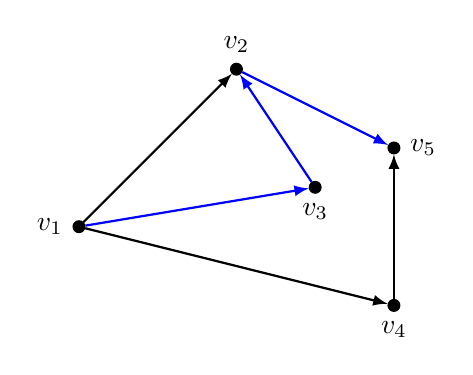
\begin{tikzpicture}

      \tikzset{enclosed/.style={draw, circle, inner sep=0pt, minimum size=.15cm, fill=black}}
%% Vertices
      	\node[enclosed, label={left: $v_1$}] (v1) at (0,2) {};
      	\node[enclosed, label={below: $v_3$}] (v2) at (3,2.5) {};
    		\node[enclosed, label={below: $v_4$}] (v3) at (4,1) {};
  	    \node[enclosed, label={above: $v_2$}] (v4) at (2,4) {};
     	\node[enclosed, label={right: $v_5$}] (v5) at (4,3) {};
%Edges
		\path [->, >=latex, thick, blue](v1) edge node[midway, sloped, above] {} (v2);
		\path [->, >=latex, thick](v1) edge node[midway, sloped, above] {} (v3);
		\path [->, >=latex, thick](v1) edge node[midway, above] {} (v4);
		\path [->, >=latex, thick, blue](v2) edge node[near end, sloped, below] {} (v4);
		\path [->, >=latex, thick](v3) edge node[midway, below] {} (v5);
		\path [->, >=latex, thick, blue](v4) edge node[near end, sloped, above] {} (v5);

	\end{tikzpicture}
	\caption{Eksempel på en orienteret simpel graf og en vej fra $v_{1}$ til $v_{5}$}
	\label{fig.vaegtetopg}
\end{figure}

Da vægtede grafer har en numerisk vægt på hver kant, kan man således beregne \emph{distancen} fra en knude til en anden i grafen. Distancen fra en knude til en anden kan defineres således:

\begin{defn}[Distance]
Lad $m\in \N $, $G=(V,E,w)$ være en vilkårlig graf og  $e_{v_i,v_{i+1}}$ være en kant, som er incident med $v_i$ og $v_{i+1}$. Lad en tilfældig, simpel vej, $P$, gå igennem knuderne således $P=(v_{1},v_{2},\dotsc,v_{m})$, da kan distancen beskrives som
	\begin{equation*}
	\mathrm{dist}(P)=\sum_{i=1}^{m}w(e_{v_i,v_{i+1}}).
	\end{equation*}  
\end{defn}

Man kan således bruge følgende definitioner af \emph{korteste vej} og \emph{længste vej} i en vægtet graf:


\begin{defn} [Korteste vej i vægtet graf]\label{defn:min.vej}
Lad $G=(V,E,w)$ være en vilkårlig, vægtet graf. Da er distancen af den korteste vej, fra en knude, $v_1$, til en anden knude, $v_m$, defineret som
	\begin{equation*}
		\alpha(v_1,v_m)=\arg \min_{P \in \euscr{P}}
		\textrm{dist}(P),
	\end{equation*}
	hvor $\euscr{P}$ er mængden af alle veje fra $v_1$ til $v_m$.
\end{defn}

På samme vis defineres længste vej:

\begin{defn} [Længste vej i en vægtet graf]
	Lad $G=(V,E,w)$ være en vilkårlig, vægtet graf. Da er distancen af den længste vej, fra en knude, $v_1$, til en anden knude, $v_m$, defineret som
	\begin{equation*}
		\beta(v_1,v_m)=\arg \max_{P \in \euscr{P}}
		\textrm{dist}(P),
	\end{equation*}
	hvor $\euscr{P}$ er mængden af alle veje fra $v_1$ til $v_m$.
\end{defn}

\begin{exmp}
Betragt figur \ref{fig.vaegtetopg} \\
\begin{figure}[H]
\centering
	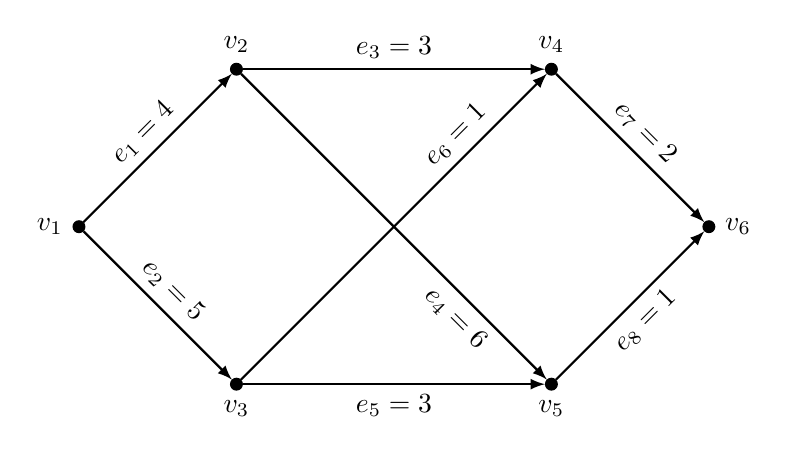
\begin{tikzpicture}

      \tikzset{enclosed/.style={draw, circle, inner sep=0pt, minimum size=.15cm, fill=black}}
%% Vertices
      	\node[enclosed, label={left: $v_1$}] (v1) at (0,2) {};
      	\node[enclosed, label={above: $v_2$}] (v2) at (2,4) {};
    	\node[enclosed, label={below: $v_3$}] (v3) at (2,0) {};
  	    \node[enclosed, label={above: $v_4$}] (v4) at (6,4) {};
     	\node[enclosed, label={below: $v_5$}] (v5) at (6,0) {};
     	\node[enclosed, label={right: $v_6$}] (v6) at (8,2) {};
%Edges
		\path [->, > = latex, thick] (v1) edge node[midway, sloped, above] {$e_1=4$} (v2);
		\path [->, > = latex, thick] (v1) edge node[midway, sloped, above] {$e_2=5$} (v3);
		\path [->, > = latex, thick] (v2) edge node[midway, above] {$e_3=3$} (v4);
		\path [->, > = latex, thick] (v2) edge node[near end, sloped, below] {$e_4=6$} (v5);
		\path [->, > = latex, thick] (v3) edge node[midway, below] {$e_5=3$} (v5);
		\path [->, > = latex, thick] (v3) edge node[near end, sloped, above] {$e_6=1$} (v4);
		\path [->, > = latex, thick] (v4) edge node[midway, sloped, above] {$e_7=2$} (v6);
		\path [->, > = latex, thick] (v5) edge node[midway, sloped, below] {$e_8=1$} (v6);

	\end{tikzpicture}
	\caption{En simpel, orienteret og vægtet graf.}
	\label{fig.vaegtetopg}
\end{figure}


På figuren ses en graf med vægtede kanter. Vi er interesserede i at finde den korteste vej fra $v_1$ til $v_6$. For at finde den korteste vej, kigger vi på alle de mulige veje fra $v_1$ til $v_6$.
Følgende veje ses:
\begin{align*}
	P_1=&(v_1,v_2,v_4,v_6)\\
	P_2=&(v_1,v_2,v_5,v_6)\\
	P_3=&(v_1,v_3,v_5,v_6)\\
	P_4=&(v_1,v_3,v_4,v_6)
\end{align*}
Man kan nu beregne distancen af de fire veje, ved at tage summen af de kanter, vejen følger. Man får derved:
\begin{align*}
	P_1=&4+3+2=9\\
	P_2=&4+6+1=11\\
	P_3=&5+3+1=9\\
	P_4=&5+1+2=8
\end{align*}
Det ses, at den korteste vej fra $v_1$ til $v_6$ er $P_4$. 
Det er sådan, man kan finde korteste vej i en vægtet graf. Denne metode kaldes \emph{brute force}. Metoden kan blive meget tidskrævende ved mere komplekse grafer. I disse tilfælde vil man bruge alternative, bedre algoritmer til at løse problemet. Dette vil vi komme ind på senere i kapitel \ref{kap.algo}.
\end{exmp}


